\documentclass{cshwk}

\begin{document}

\title{HW \#2, Chapter 2}

\maketitle

\section*{Problem 1. Chapter 2 P 18}

\begin{enumerate}
    \renewcommand{\labelenumi}{(\alph{enumi})}
    \item What is a whois database?
    \item Use various whois databases on the Internet to obtain the names of two DNS servers. Indicate which whois databases you used.
    \item Use \texttt{nslookup} on your local host to send DNS queries to three DNS servers: your local DNS server and the two DNS servers you found in part (b). Try querying for Type A, NS, and MX reports. Summarize your findings.
    \item Use \texttt{nslookup} to find a Web server that has multiple IP addresses. Does the Web server of your institution (school or company) have multiple IP addresses?
    \item Use the ARIN whois database to determine the IP address range used by your university.
    \item Describe how an attacker can use whois databases and the \texttt{nslookup} tool to perform reconnaissance on an institution before launching an attack.
    \item Discuss why whois databases should be publicly available.
\end{enumerate}

\subsection*{Solutions:}

\subsubsection*{a. What is a whois database?}

A whois database is a publicly accessible resource that contains detailed information about domain names, IP address ranges, and autonomous systems. It is commonly used to look up information about the ownership of a domain name, the associated IP address range, and the autonomous system number (ASN).

\subsubsection*{b. Use various whois databases on the Internet to obtain the names of two DNS servers. Indicate which whois databases you used.}

I used the \texttt{ICANN WHOIS} database to retrieve the DNS server information for \href{https://www.google.com}{google.com} and \href{https://www.facebook.com}{facebook.com}. The results are shown in Fig.~\ref{fig:whois-icann-google} through Fig.~\ref{fig:whois-icann-facebook}, as well as in Tab.~\ref{tab:whois-icann}.


\begin{figure}[htbp]
    \centering
    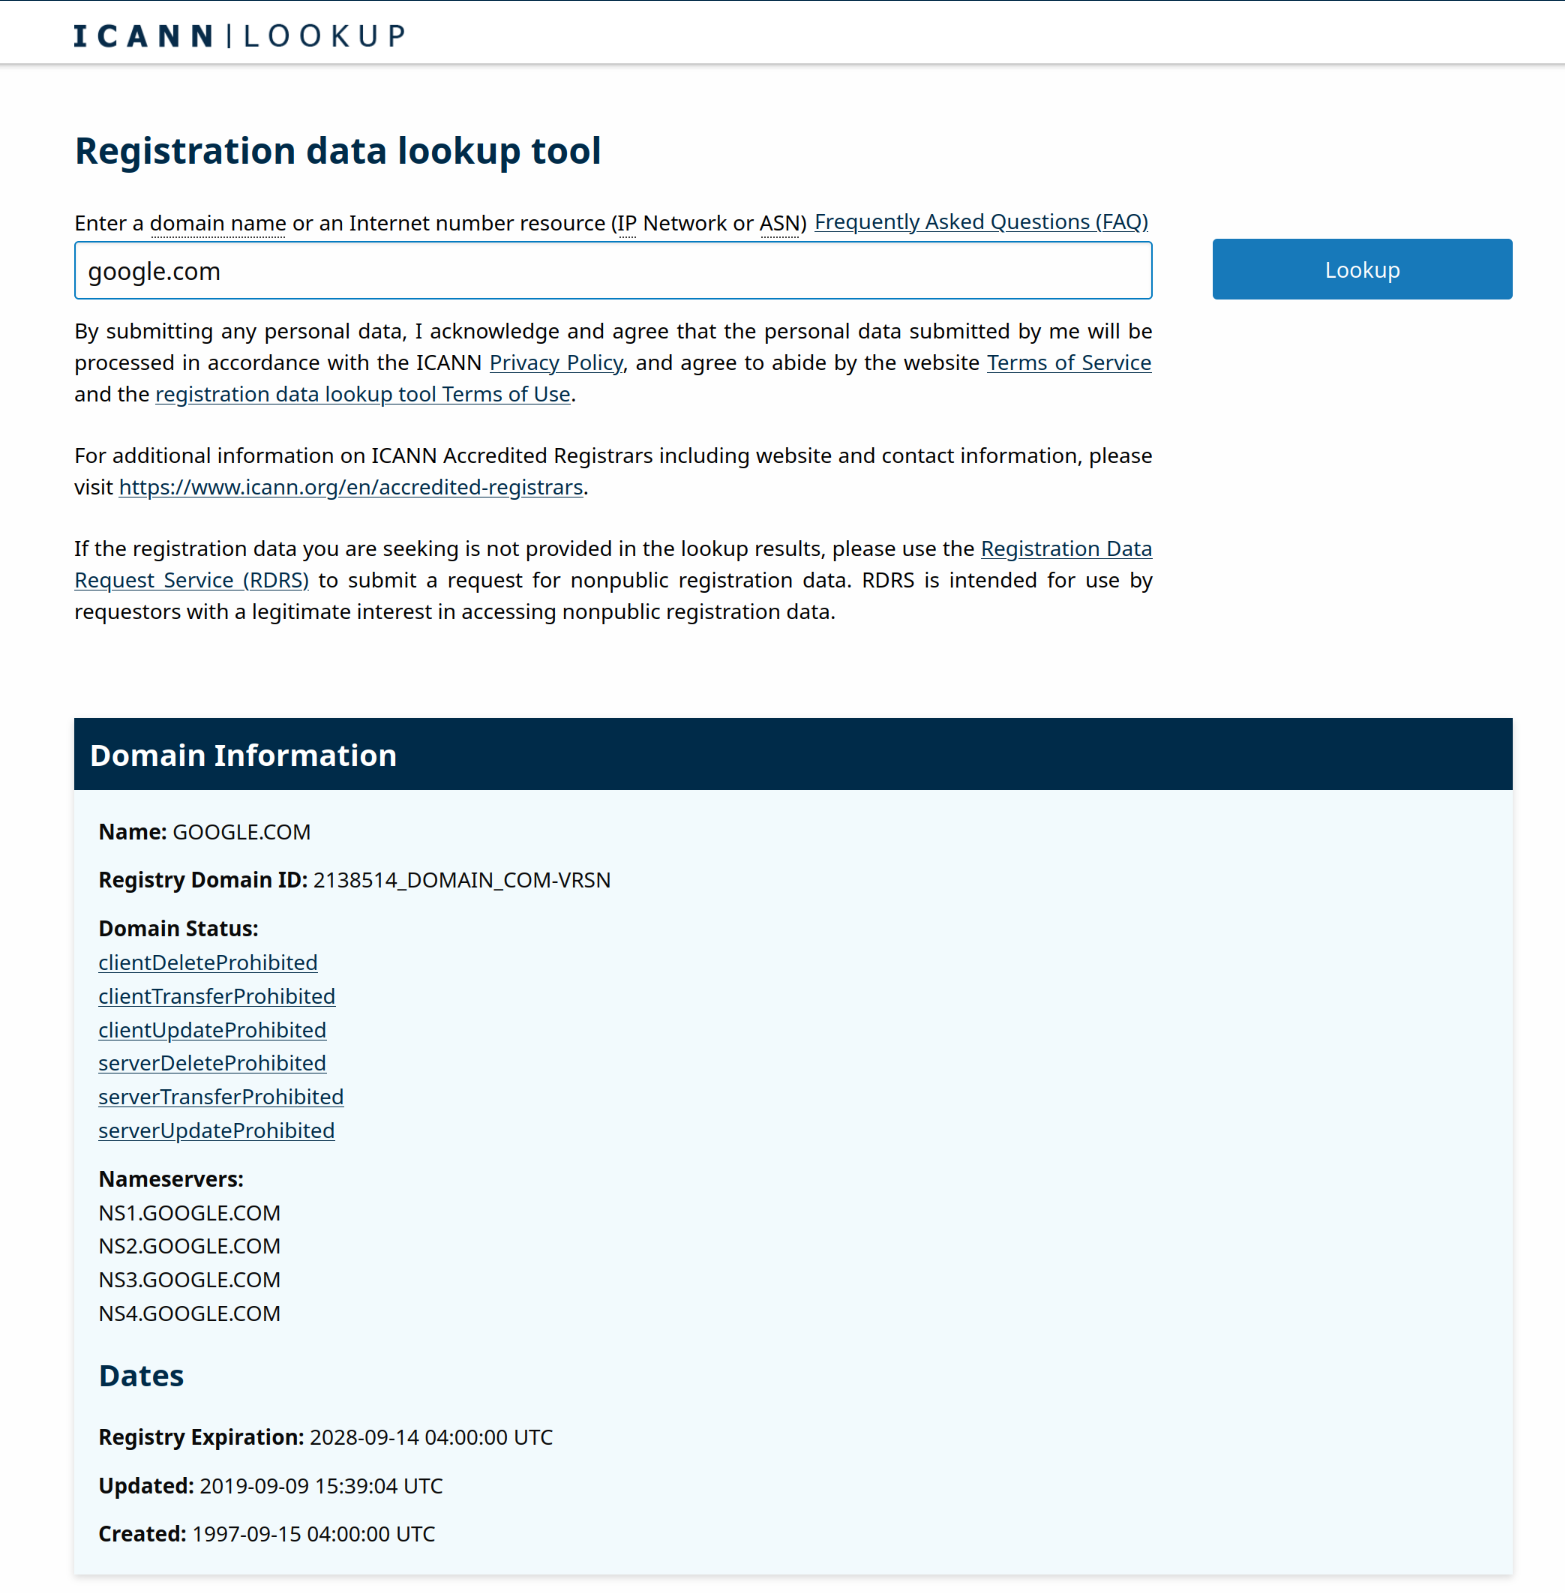
\includegraphics[width=0.8\textwidth]{hw2-1-1.png}
    \caption{ICANN WHOIS database result for google.com}
    \label{fig:whois-icann-google}
\end{figure}

\begin{figure}[htbp]
    \centering
    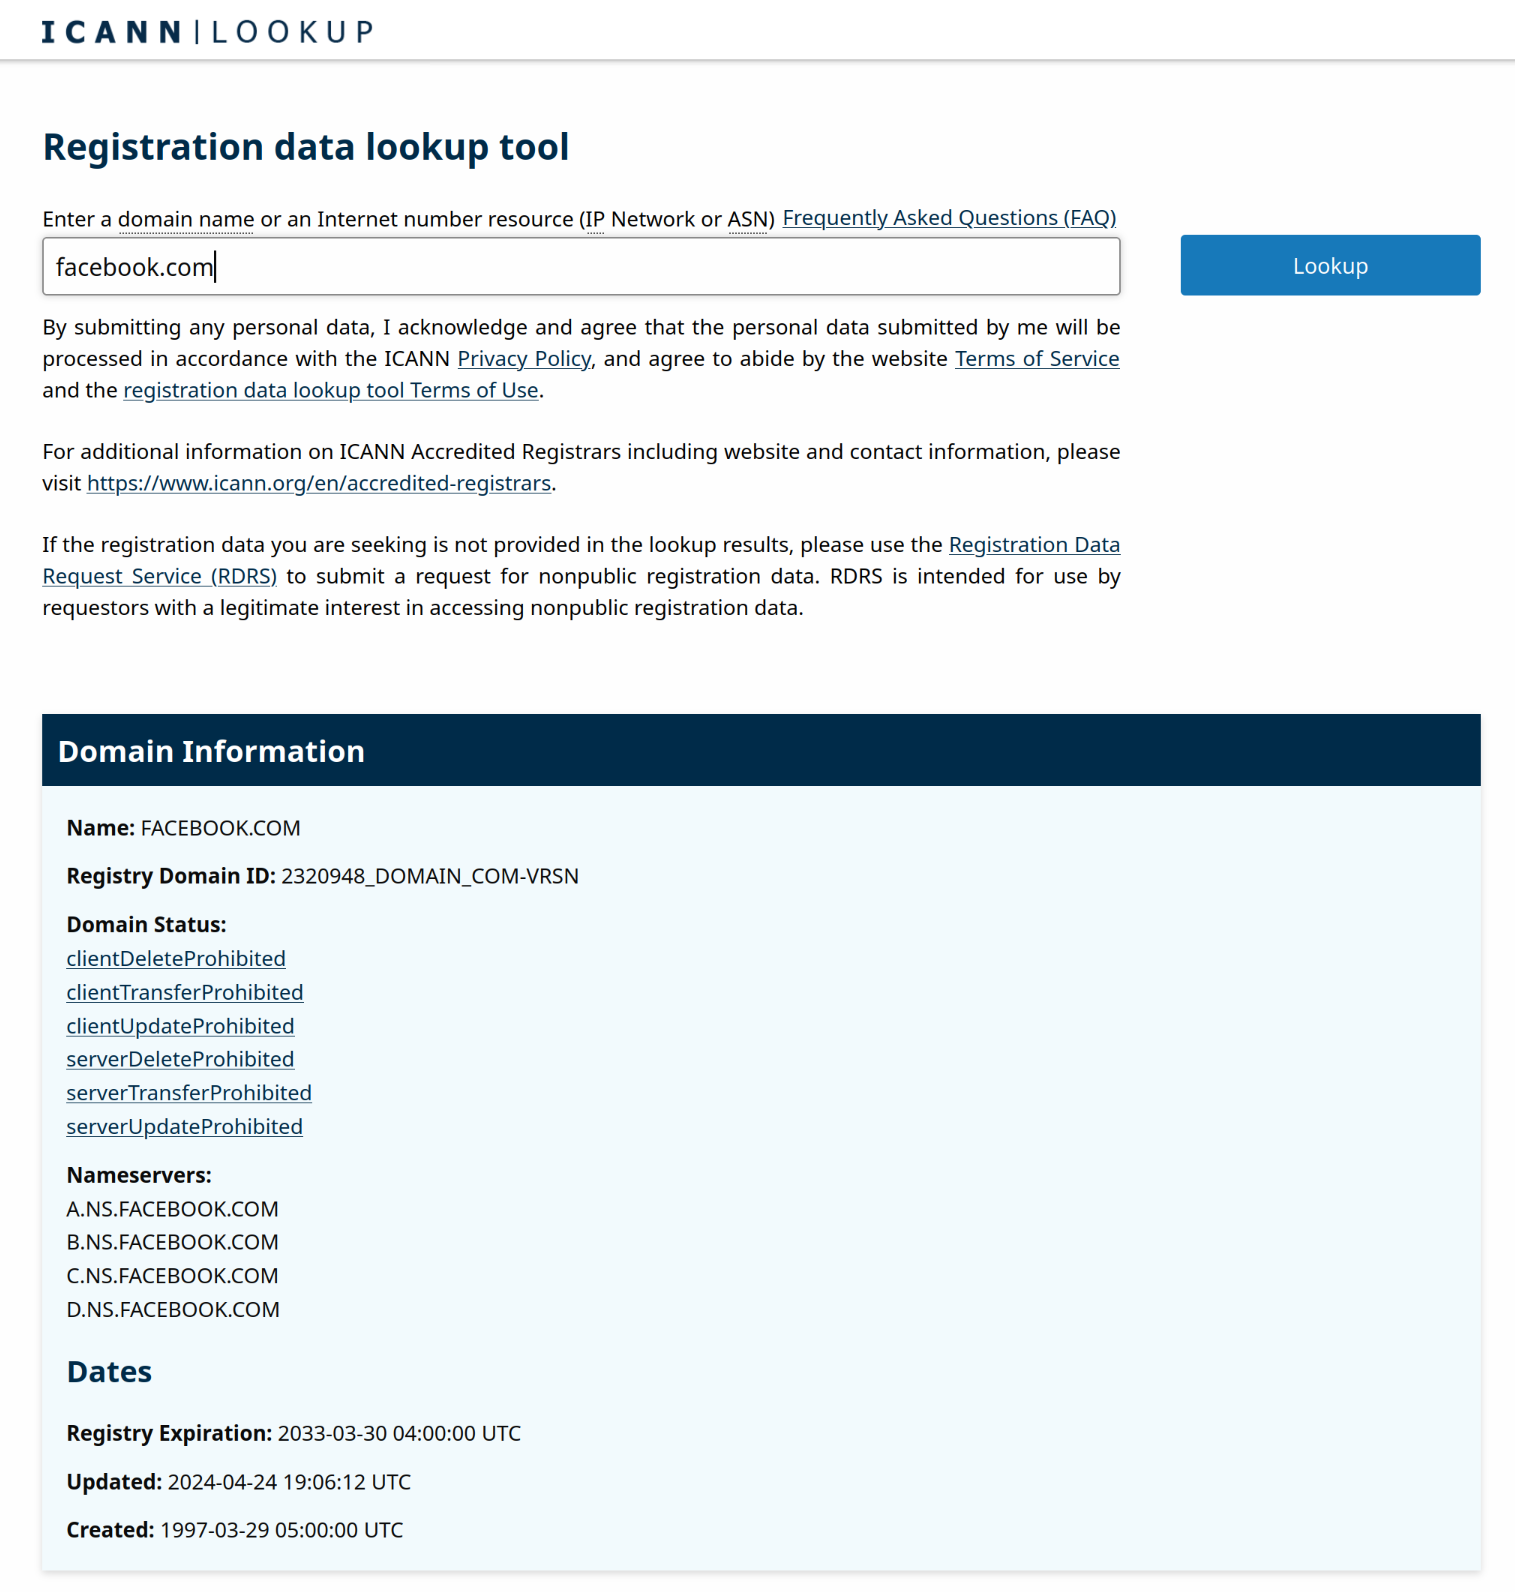
\includegraphics[width=0.8\textwidth]{hw2-1-2.png}
    \caption{ARIN WHOIS database result for google.com}
    \label{fig:whois-icann-facebook}
\end{figure}

\begin{table}[htbp]
    \centering
    \begin{tabular}{cl}
        \hline
        Domain                        & DNS Server        \\
        \hline
        \multirow{4}{*}{google.com}   & ns1.google.com    \\
                                      & ns2.google.com    \\
                                      & ns3.google.com    \\
                                      & ns4.google.com    \\
        \hline
        \multirow{4}{*}{facebook.com} & a.ns.facebook.com \\
                                      & b.ns.facebook.com \\
                                      & c.ns.facebook.com \\
                                      & d.ns.facebook.com \\
        \hline
    \end{tabular}
    \caption{DNS servers for google.com and facebook.com}
    \label{tab:whois-icann}
\end{table}
\subsubsection*{c. Use \texttt{nslookup} on your local host to send DNS queries to three DNS servers: your local DNS server and the two DNS servers you found in part (b). Try querying for Type A, NS, and MX records. Summarize your findings.}

To query DNS records for a target domain using \texttt{nslookup}, you can run the following command:

\begin{verbatim}
    nslookup -type=<record_type> <domain> <dns_server,optional>
\end{verbatim}

First, we ran \texttt{nslookup} on the local DNS server. The results are displayed in Fig.~\ref{fig:nslookup-local}.

\begin{lstlisting}
    nslookup -type=A google.com
    nslookup -type=NS google.com
    nslookup -type=MX google.com
\end{lstlisting}

\begin{figure}[htbp]
    \centering
    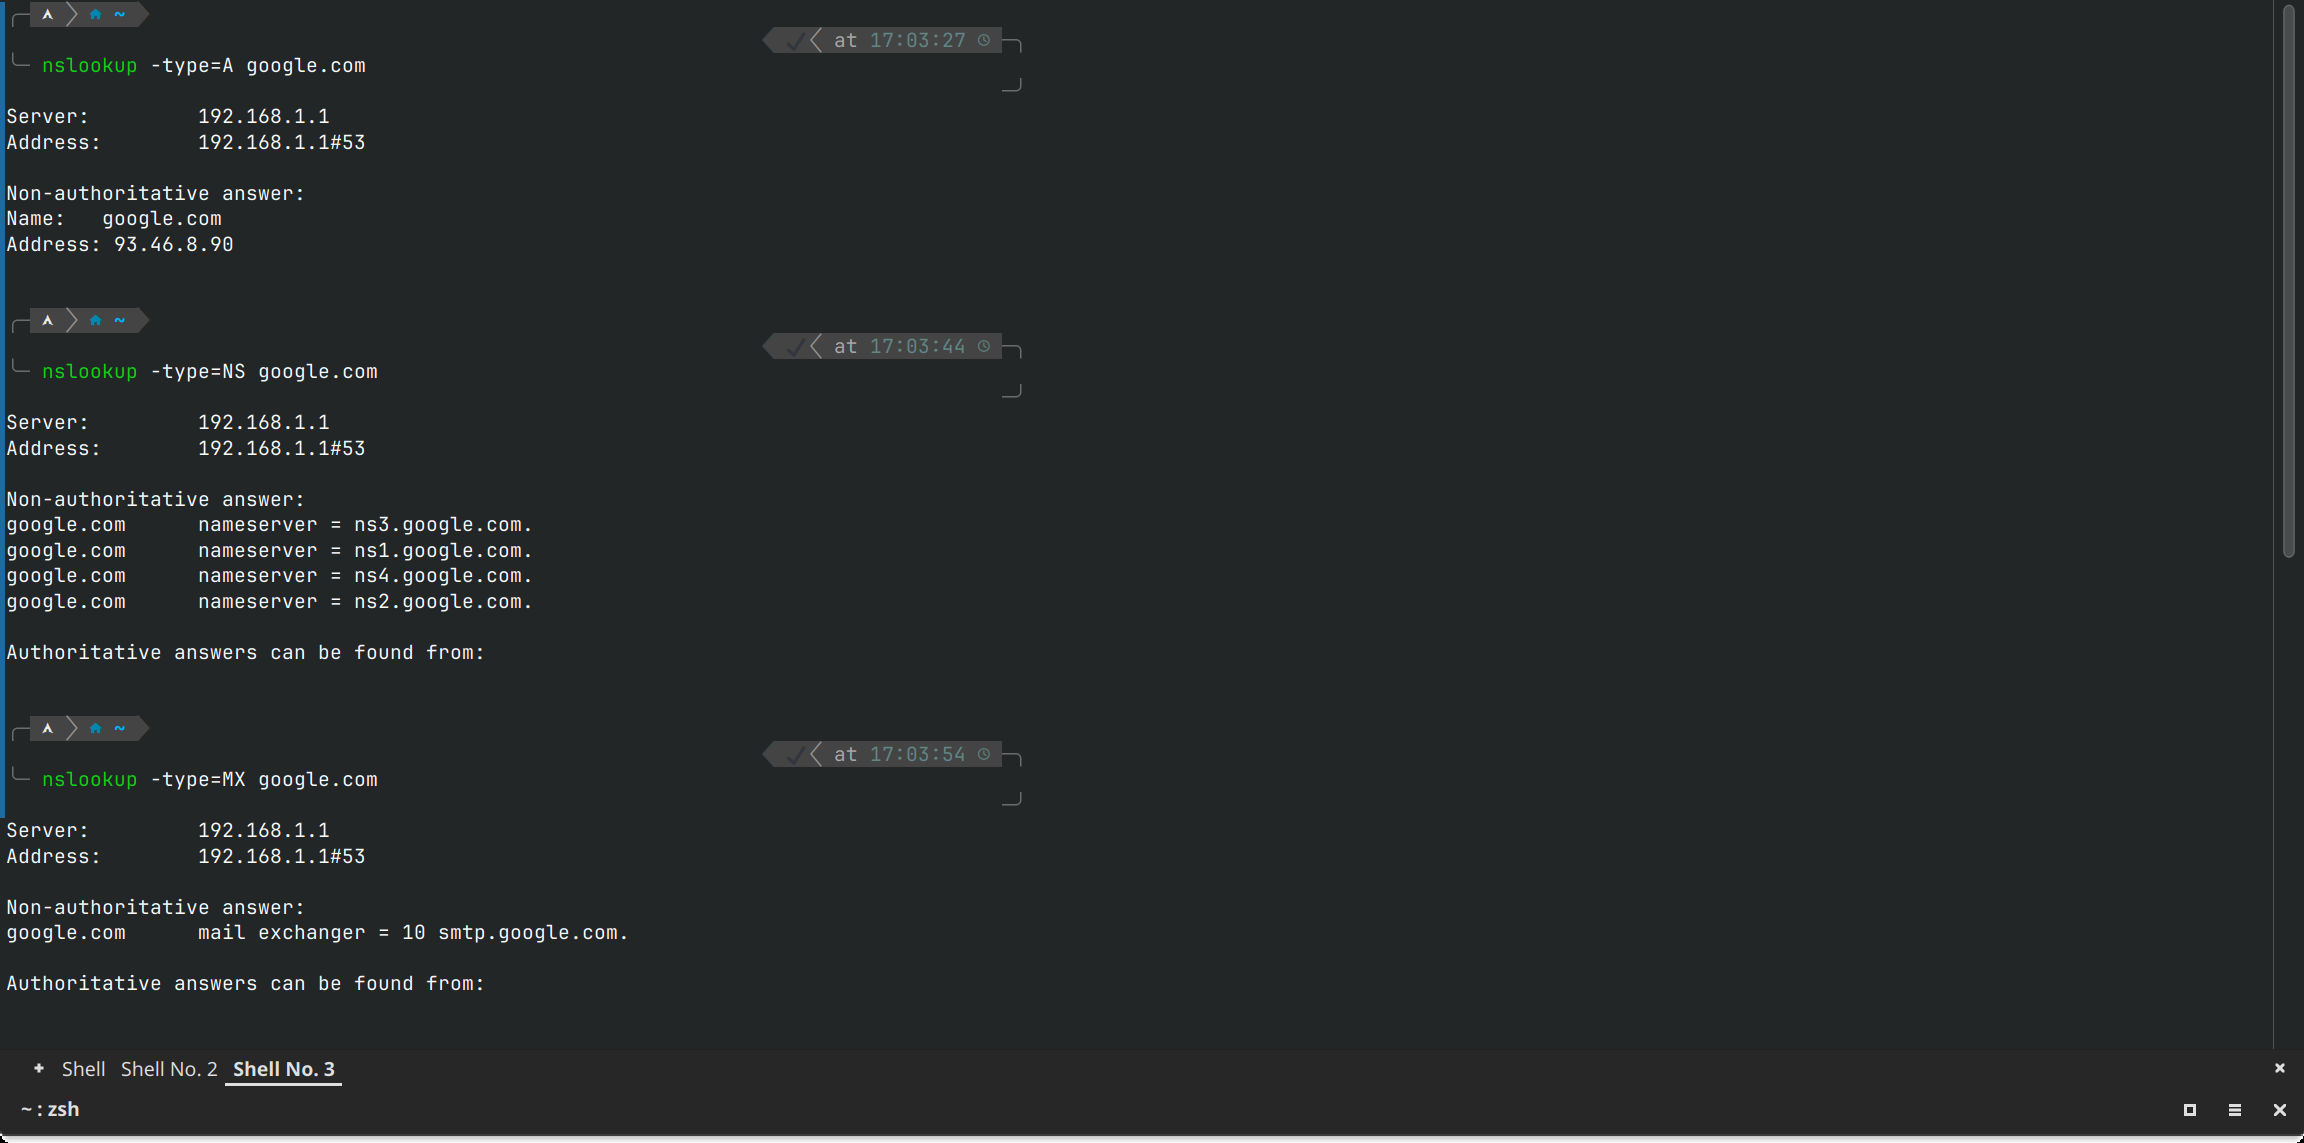
\includegraphics[width=0.8\textwidth]{hw2-1-3.png}
    \caption{nslookup results for local DNS server}
    \label{fig:nslookup-local}
\end{figure}


Second, we ran \texttt{nslookup} on \texttt{ns1.google.com}, and the results are shown in Fig.~\ref{fig:nslookup-google}.


\begin{lstlisting}
    nslookup -type=A google.com ns1.google.com
    nslookup -type=NS google.com ns1.google.com
    nslookup -type=MX google.com ns1.google.com
\end{lstlisting}

\begin{figure}[htbp]
    \centering
    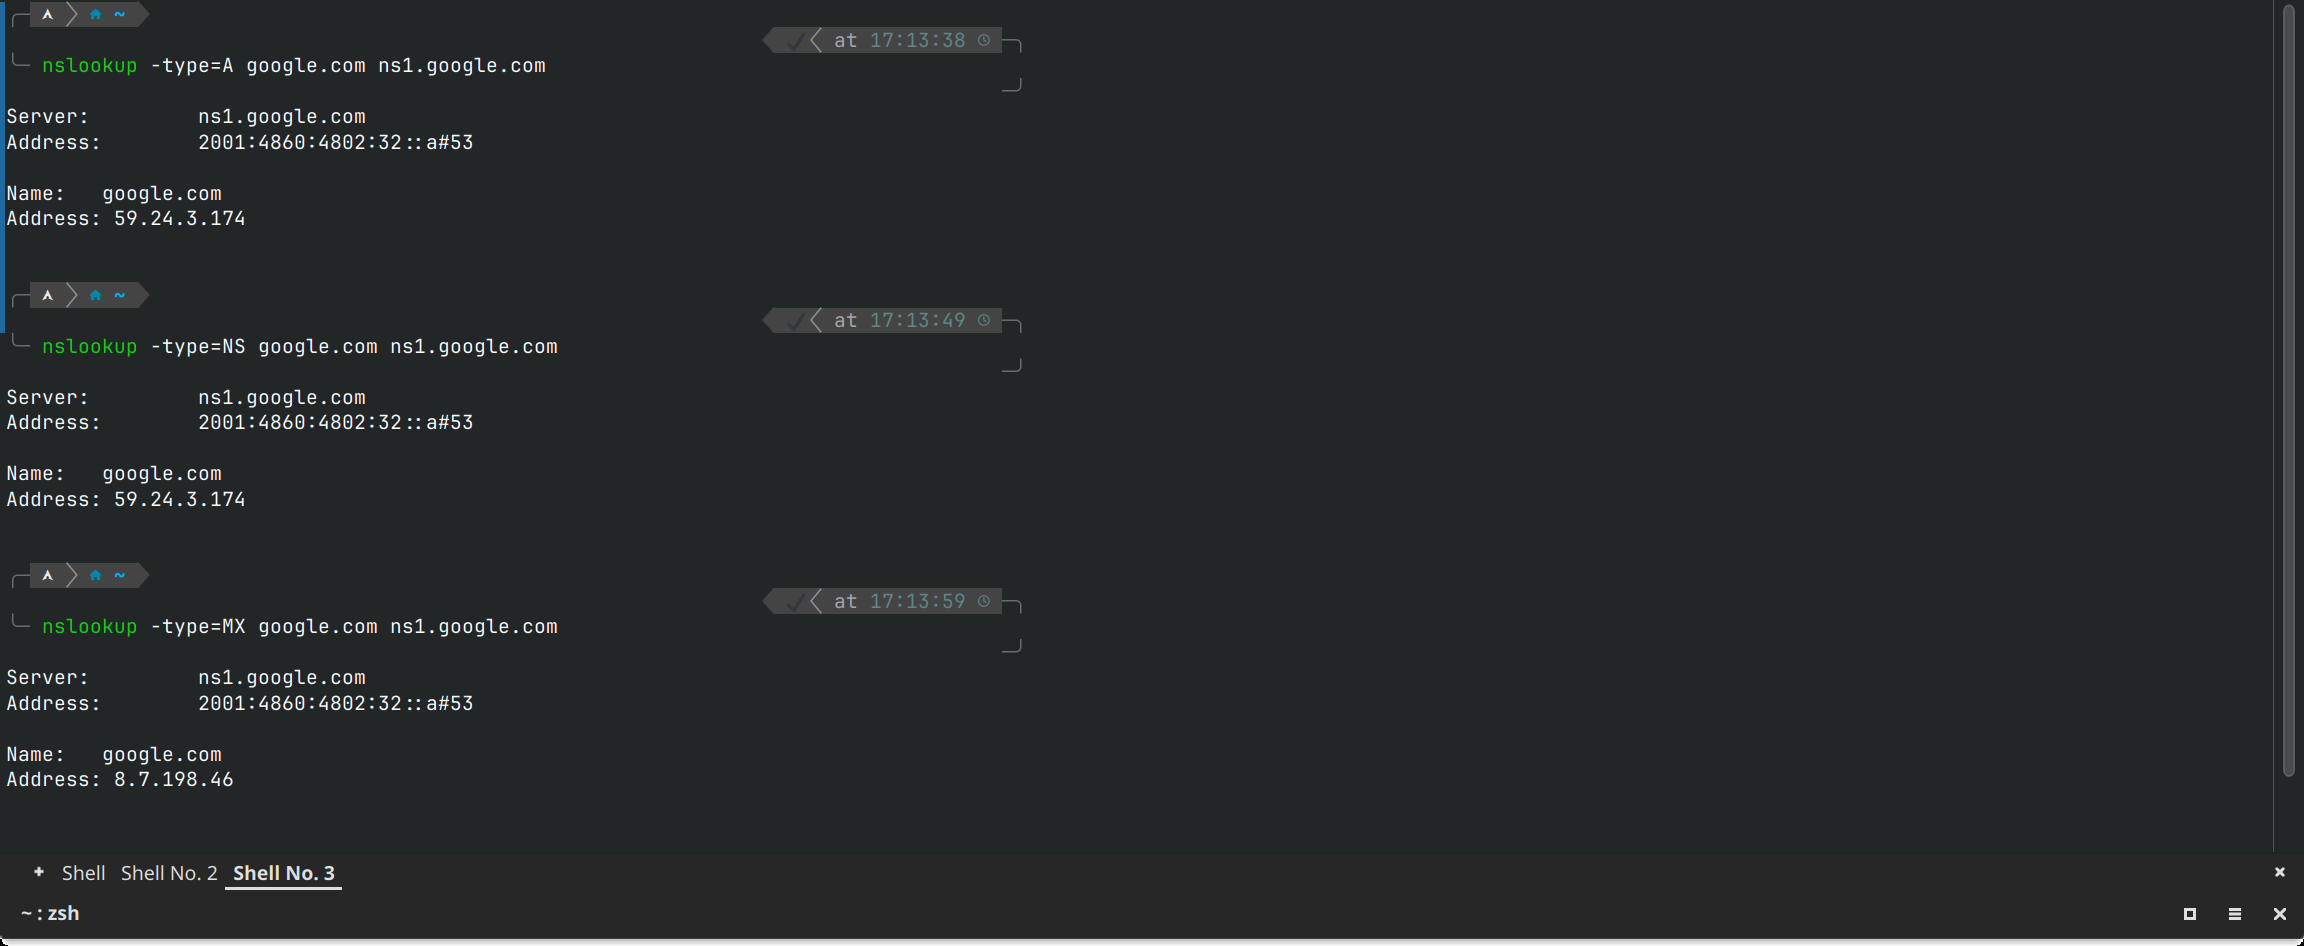
\includegraphics[width=0.8\textwidth]{hw2-1-4.png}
    \caption{nslookup results for ns1.google.com}
    \label{fig:nslookup-google}
\end{figure}

Third, we ran \texttt{nslookup} on \texttt{ns2.google.com}, which is another DNS server for Google. The results are displayed in Fig.~\ref{fig:nslookup-facebook}.


\begin{lstlisting}
    nslookup -type=A google.com ns2.google.com
    nslookup -type=NS google.com ns2.google.com
    nslookup -type=MX google.com ns2.google.com
\end{lstlisting}

\begin{figure}[htbp]
    \centering
    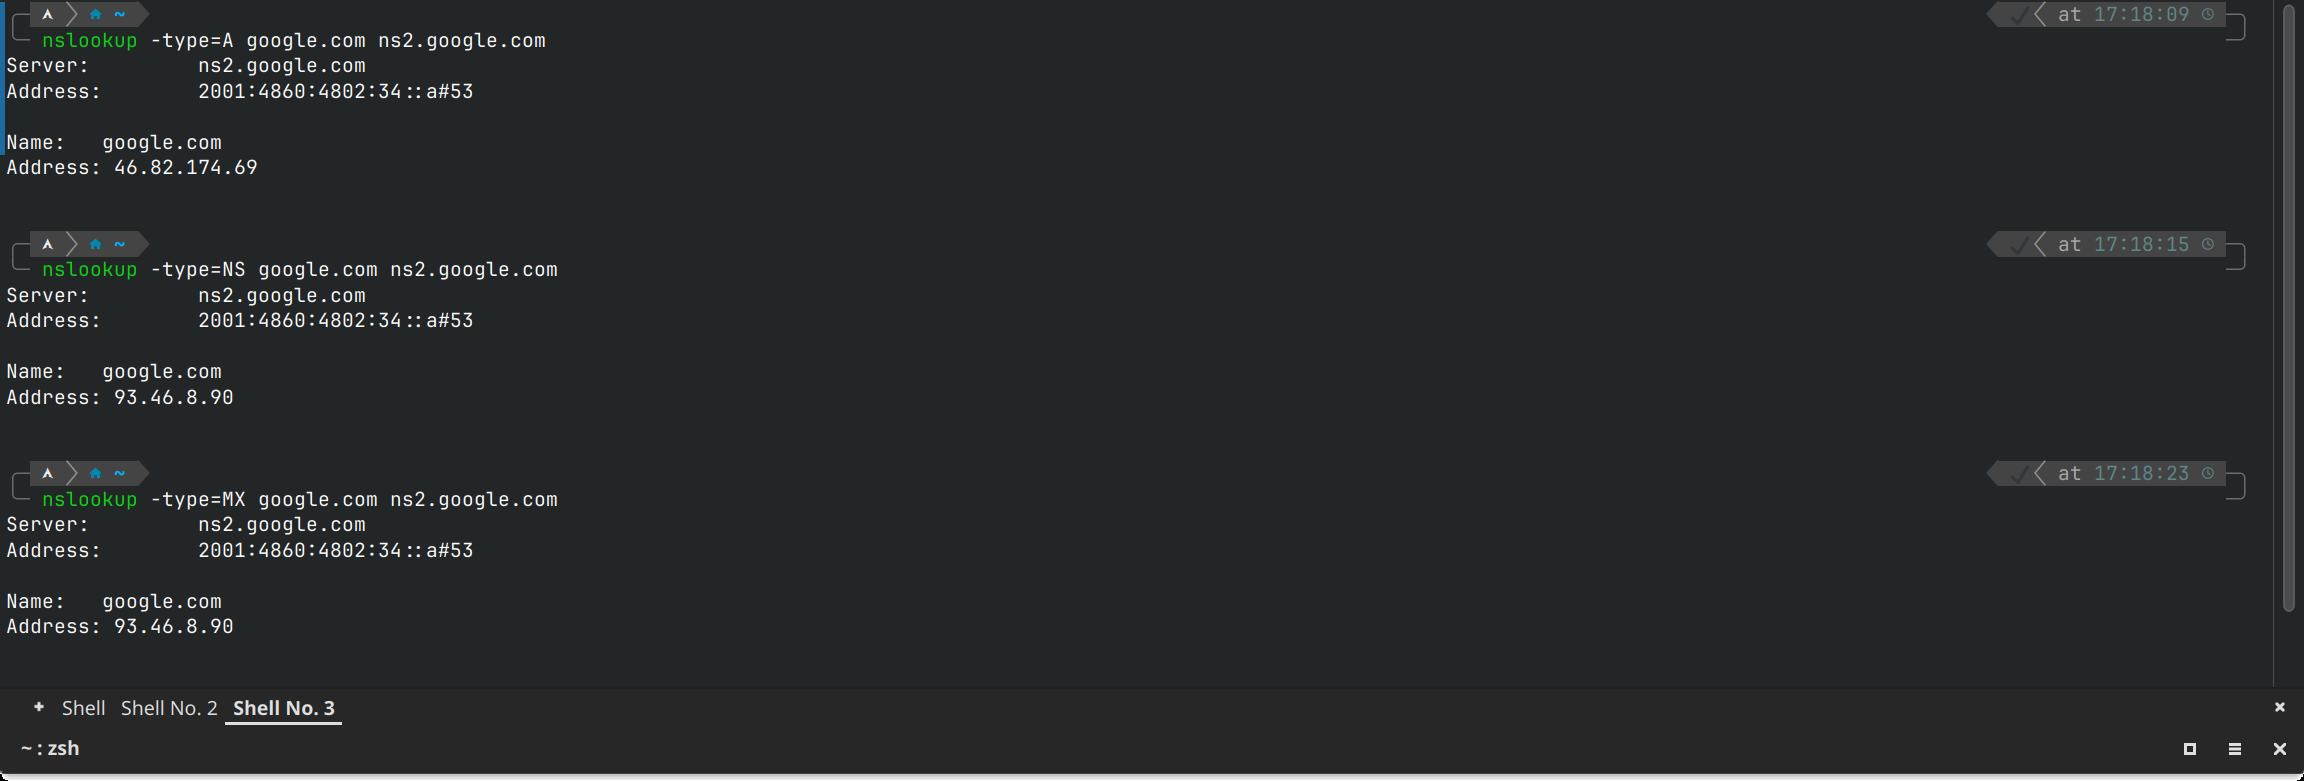
\includegraphics[width=0.8\textwidth]{hw2-1-5.png}
    \caption{nslookup results for ns2.google.com}
    \label{fig:nslookup-facebook}
\end{figure}

Now, let's inspect and summarize the results from the three DNS servers. The detailed results are presented in Tab.~\ref{tab:nslookup}.


\begin{table}[htbp]
    \centering
    \begin{tabular}{cccc}
        \hline
        DNS Server     & Type A       & Type NS            & Type MX         \\
        \hline
        Local DNS      & 93.46.8.90   & ns[1-4].google.com & smtp.google.com \\
        ns1.google.com & 59.24.3.174  & 59.24.3.174        & 8.7.198.46      \\
        ns2.google.com & 46.82.174.69 & 93.46.8.90         & 93.46.8.90      \\
        \hline
    \end{tabular}
    \caption{nslookup results for google.com}
    \label{tab:nslookup}
\end{table}

From the image and results, we can see that the local DNS server provides a **Non-authoritative answer** for all DNS records. This happens because the local DNS server is caching the results from the authoritative server.

Additionally, by examining the IP addresses in each report, we notice that the Type A records vary across different DNS servers. This is due to large websites like Google using multiple servers for load balancing and fault tolerance. Moreover, the Type NS records from `ns2.google.com` match those of the local DNS server, further confirming that the local DNS server is caching results from the authoritative server.

\subsubsection*{d. Use \texttt{nslookup} to find a web server that has multiple IP addresses. Does your institution's web server (school or company) have multiple IP addresses?}

\texttt{Google} is an example of a website with multiple IP addresses, as shown in Tab.~\ref{tab:nslookup}.

Next, let’s examine the official website of Tianjin University, \href{tju.edu.cn}{https://tju.edu.cn}, using Google's DNS server \texttt{8.8.8.8}. The results are shown in Fig.~\ref{fig:nslookup-tju}.


\begin{verbatim}
    nslookup -type=A tju.edu.cn 8.8.8.8
\end{verbatim}

\begin{figure}[htbp]
    \centering
    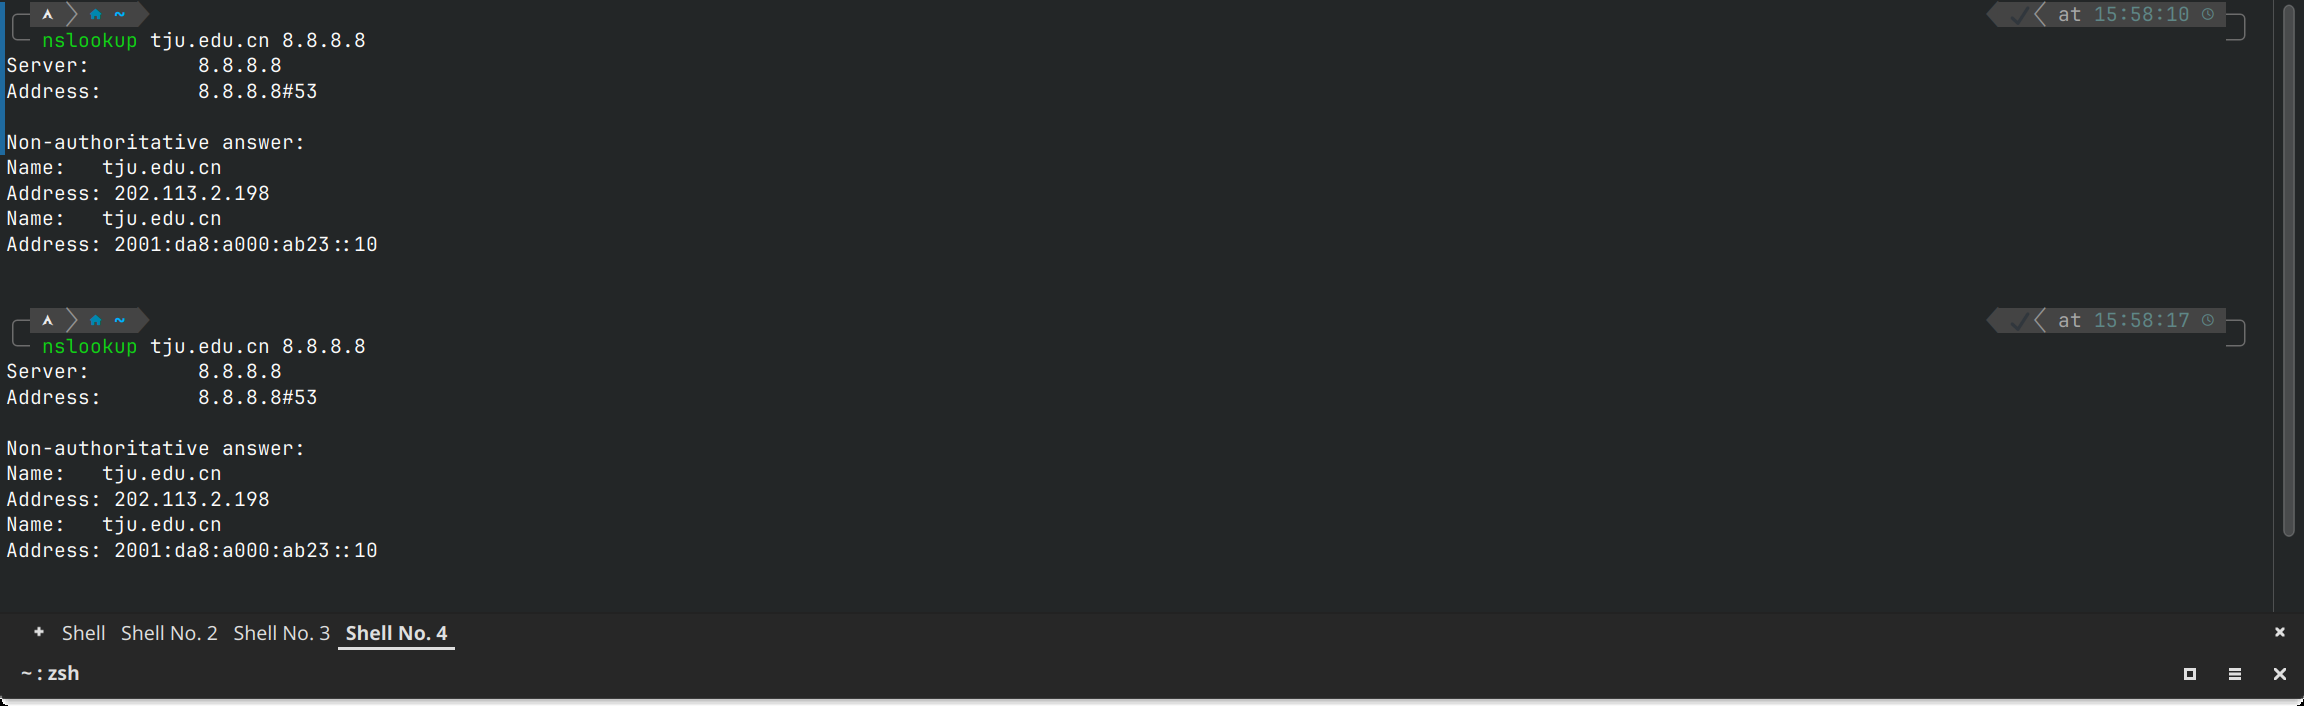
\includegraphics[width=0.8\textwidth]{hw2-1-6.png}
    \caption{nslookup results for tju.edu.cn}
    \label{fig:nslookup-tju}
\end{figure}

Execute the command multiple times, it returns the same IP address which is \texttt{202.113.2.198}. This indicates that the official website of Tianjin University does not have multiple IP addresses, which is reasonable because the server of the official website is at the same location in the campus and shares the same \texttt{IPv4} Addresss.

\subsubsection*{e. Use the ARIN whois database to determine the IP address range used by your university.}

Tianjin University is located in Tianjin, China, and is registered through \texttt{CERNET}. Therefore, the ARIN whois database does not contain information about Tianjin University. Instead, we can use the \texttt{CERNET} whois database to find the IP address range used by Tianjin University. However, as of \today, the \texttt{CERNET} whois database \url{https://web.nic.edu.cn/cgi-bin/reg/otherobj} is not available and returns Error Code \texttt{403}, as shown in Fig.~\ref{fig:whois-cernet}.

\begin{figure}[htbp]
    \centering
    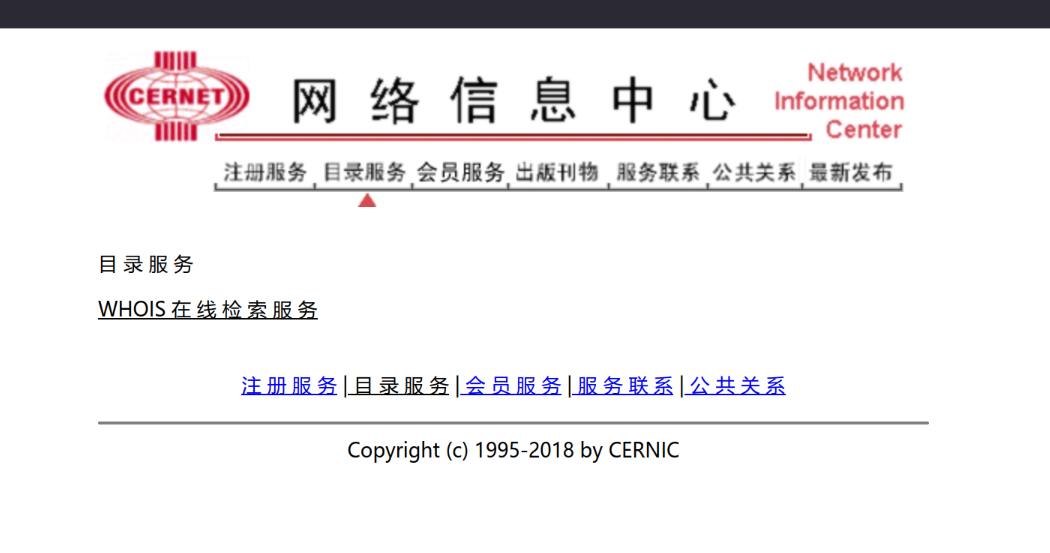
\includegraphics[width=0.8\textwidth]{hw2-1-7.png}
    \caption{CERNET WHOIS database result for tju.edu.cn}
    \label{fig:whois-cernet}
\end{figure}

Instead, Use \texttt{CNNIC} to check the \texttt{whois} information of \href{https://subit.org.cn}{subit.org.cn}, which is my personal domain to show the process. The results are shown in Fig.~\ref{fig:whois-cnnic}.

\begin{figure}[htbp]
    \centering
    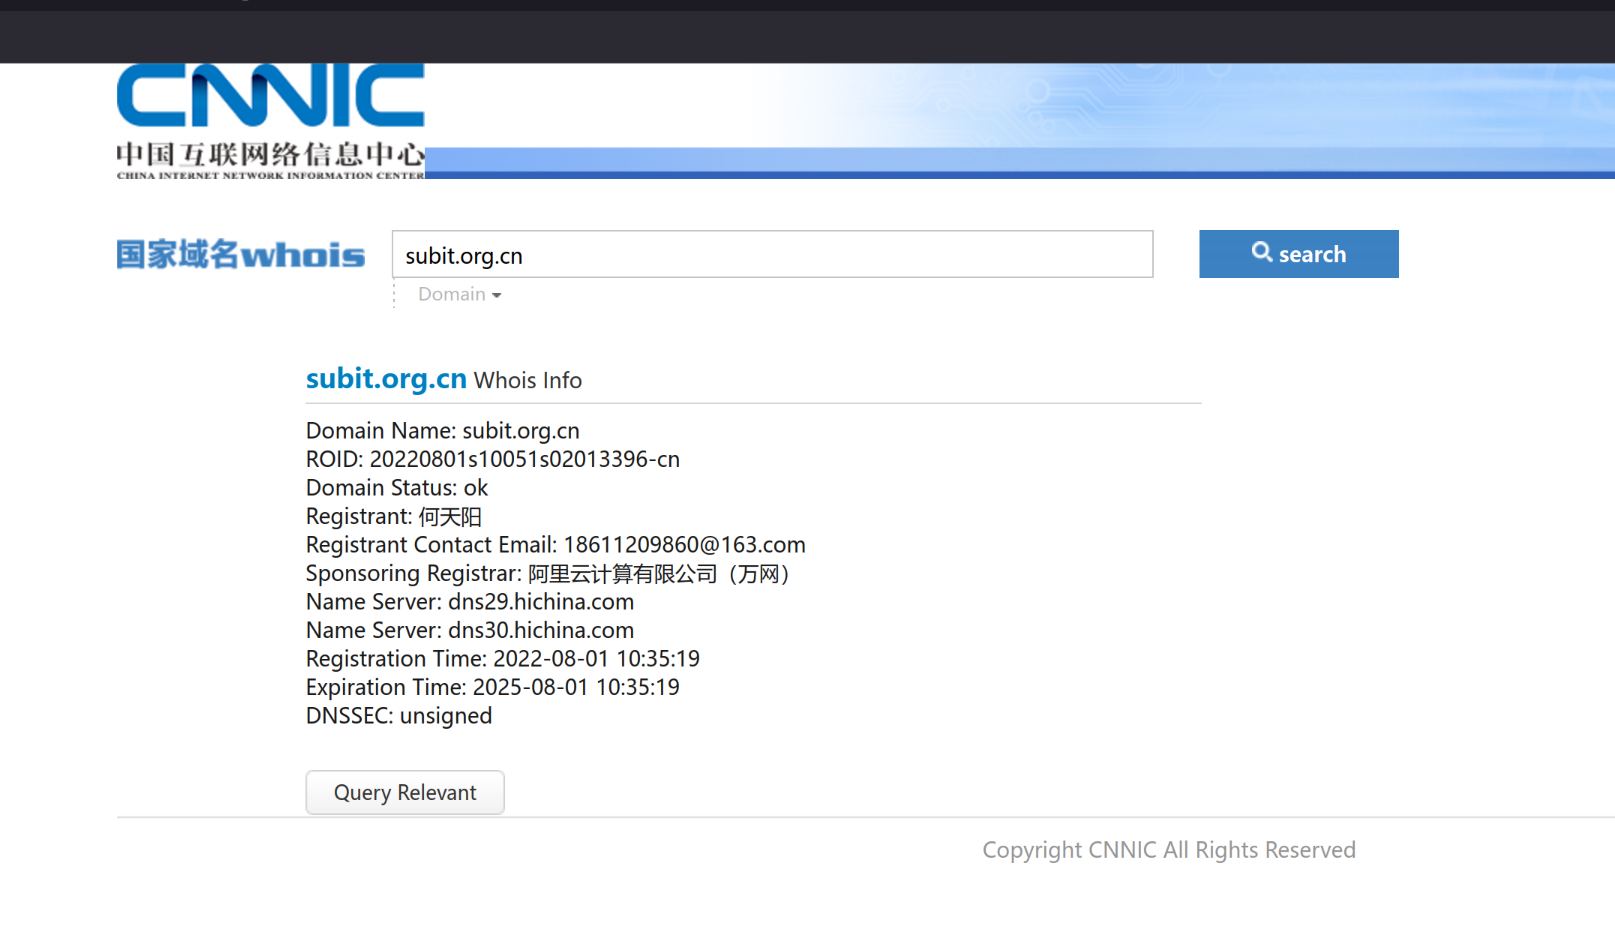
\includegraphics[width=0.8\textwidth]{hw2-1-8.png}
    \caption{CNNIC WHOIS database result for subit.org.cn}
    \label{fig:whois-cnnic}
\end{figure}

\subsubsection*{f. Describe how an attacker can use whois databases and the \texttt{nslookup} tool to perform reconnaissance on an institution before launching an attack.}

An attacker can use whois databases and the \texttt{nslookup} tool to gather valuable information about an institution’s domain and network infrastructure. By querying a whois database, the attacker can retrieve details about the domain, such as the registrar, registration and expiration dates, nameservers, and sometimes even contact information for the domain owner or administrative staff. This data can help the attacker determine potential weak points, like outdated domain records or vulnerable domain management practices.

The \texttt{nslookup} tool allows attackers to perform DNS lookups on domain names or IP addresses. It can provide insights into the DNS records of the institution, including IP addresses linked to the domain, the type of DNS records in use (A, MX, CNAME, etc.), and the servers responsible for the domain’s DNS resolution. By analyzing this information, the attacker can map the institution's network, identify possible entry points, or plan for DNS-related attacks like DNS spoofing or poisoning.

\subsubsection*{g. Discuss why whois databases should be publicly available.}

Whois databases should be publicly available to promote transparency and accountability on the internet. By allowing access to information about domain ownership, individuals and organizations can verify the legitimacy of websites and domains, reducing the risk of online fraud or abuse. Public access to whois data can also assist in resolving domain-related disputes, such as intellectual property issues, as well as enabling law enforcement or security researchers to track down malicious entities responsible for cyberattacks or other illegal activities.

Moreover, public whois data facilitates network troubleshooting by providing essential details that can help administrators resolve issues related to domain misconfigurations or abuse. While privacy concerns exist, modern practices such as redacting sensitive contact information or using privacy protection services help strike a balance between transparency and personal privacy.


\end{document}